\documentclass[a4paper,11pt,dvipdfmx]{jsarticle}

\usepackage{bm}
\usepackage[dvipdfmx]{graphicx}
\usepackage[subrefformat=parens]{subcaption}
\usepackage[dvipdfmx]{color}
\usepackage{ascmac}
\usepackage{siunitx}
\usepackage{otf}
\pagestyle{plain}
\usepackage{float}
\usepackage[dvipdfmx]{hyperref}
\usepackage{pxjahyper}
\usepackage{here}
\usepackage{titlesec}
\titleformat*{\section}{\LARGE\bfseries}
\titleformat*{\subsection}{\normalsize\bfseries}
\usepackage{url}
\usepackage{comment}
\usepackage[table,xcdraw]{xcolor}
\hypersetup{% hyperrefオプションリスト
setpagesize=false,
 bookmarksnumbered=true,%
 bookmarksopen=true,%
 colorlinks=true,%
 linkcolor=blue,
 citecolor=blue,
}

\begin{document}


\subsection{セットアップ}


\subsubsection{真空チェンバー}
加速器から送られてきた陽子ビームは、真空チェンバー内に誘導しターゲットに衝突させる。真空チェンバーの写真を図\ref{chanber}に、真空チェンバー内の模式図を図\ref{chanbermoshi}に示す。ターゲットは、アルミ板に張り付け又は挟まれて設置されている。真ん中にある円柱管は二次電子抑制管である。検出器には2.3節で記載するPINフォトダイオードをチャージアンプに付けたものをPINフォト台に設置し利用する。今回の研究では散乱陽子と反跳粒子の両方を検出したいため、検出器を2つ設置した。図\ref{chanbermoshi}の赤矢印のように加速器で加速した陽子を真空チェンバー内に誘導し、ターゲットに衝突させる。二次電子抑制管とビームストッパーは導通しており、電流値を測定することが出来る。また、ターゲットホルダーに当たったビームによる電流値も測定できるようになっている。真空チェンバーは真空ポンプに接続されており、10$^\text{-5}$Paの真空状態を作れるようになっている。
 
 
  \begin{figure}[H]
    \centering
    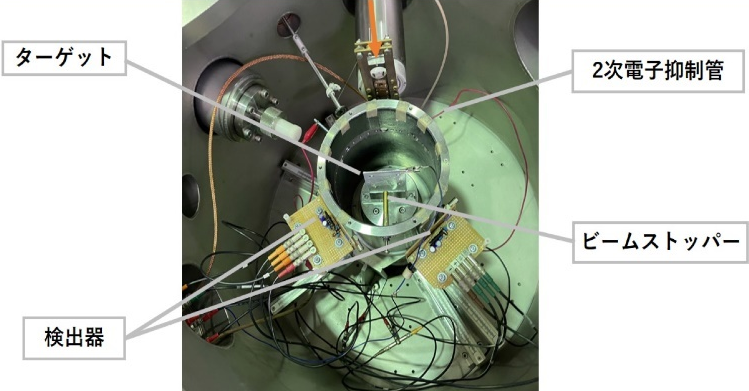
\includegraphics[width=80mm]{picture/setup/chanber.png}
    \caption{真空チェンバーの写真}
    \label{chanber}
  \end{figure}
  
  \begin{figure}[H]
    \centering
    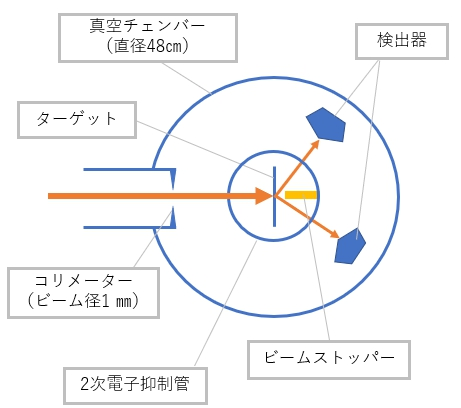
\includegraphics[width=70mm]{picture/setup/chanbermoshi.jpg}
    \caption{真空チェンバー内の模式図}
    \label{chanbermoshi}
  \end{figure}
  
\subsubsection{二次電子抑制管}
真空チェンバーの真ん中にある円柱管を二次電子抑制管という。二次電子抑制管の直径は12cmであり、10度ごとに直径3mmのネジ穴があいている。そのため10度ずつ検出器を動かして実験を行うことができる。今回利用する二次電子抑制管には、ビームストッパーの位置を軸として45度の部分に穴が開いていたため、測定の際の40度・50度への影響を考えてネジで穴を塞いでいる。また140度の穴は大きいものになっている。図\ref{yokokan}に横から見た二次電子抑制管の写真を示す。
 
  \begin{figure}[H]
    \centering
    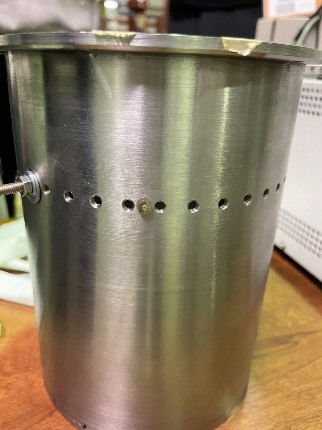
\includegraphics[width=35mm]{picture/setup/yokokan.jpg}
    \caption{横から見た二次電子抑制管の写真}
    \label{yokokan}
  \end{figure}
  
\subsubsection{ビームストッパー}
ラザフォード散乱の微分散乱断面積は、散乱の角度が小さくなるにつれて急速に増大する。そのため、散乱角$\theta=30^{\circ}$未満の散乱が二次電子抑制管で再び散乱してしまうと大きなバックグラウンドになりかねない。これを防ぐためにビームストッパーを設置する。

\par
ビームストッパーは市販の真鍮パイプを切断したものであり、これにネジを付け2次電子抑制管に設置する。長さは43mm、内径は4.5mm、厚さは1mmである。利用したビームストッパーは先行研究\cite{2019}で実績が証明されていたものを利用している。図\ref{stphoto}にビームストッパーの写真を、図\ref{stsekkei}にビームストッパーの設計図を示す。ビームストッパーは真鍮製で、厚さが1mmあるため、図\ref{stmoshi1}のようにビームを十分に止めることが出来る。図\ref{stmoshi2}のようにねじで反射したとしても、反射したビームの反射角は約3度になるため今回の測定範囲に関しては影響がない。

\begin{figure}[H]
 \begin{minipage}{0.5\hsize}
  \begin{center}
   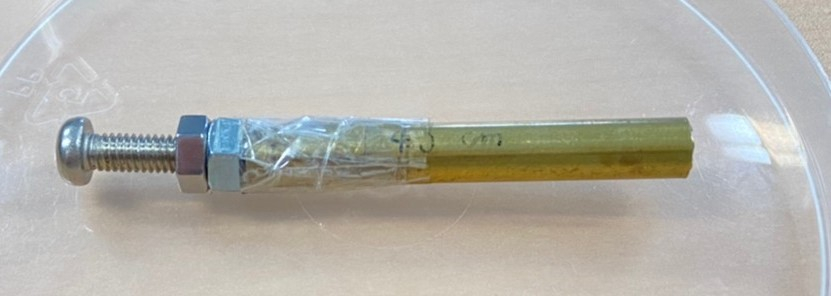
\includegraphics[width=50mm]{picture/setup/stopperphoto.jpg}
  \end{center}
  \caption{ビームストッパーの写真}
  \label{stphoto}
 \end{minipage}
 \begin{minipage}{0.5\hsize}
  \begin{center}
   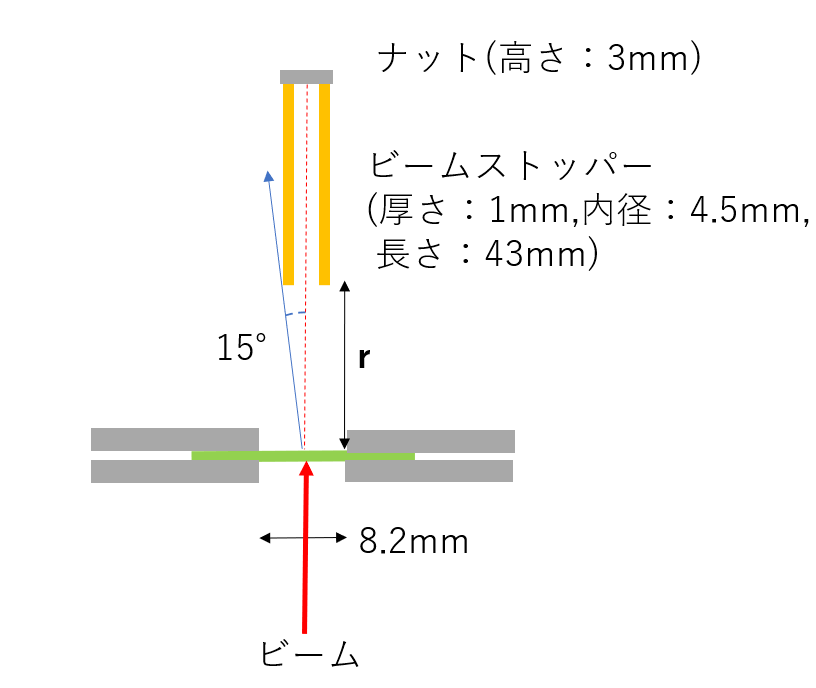
\includegraphics[width=40mm]{picture/setup/stoppersekkei.png}
  \end{center}
  \caption{ビームストッパーの設計図\cite{2019}}
  \label{stsekkei}
 \end{minipage}
\end{figure}

\begin{figure}[H]
  \begin{minipage}{0.5\hsize}
    \centering
    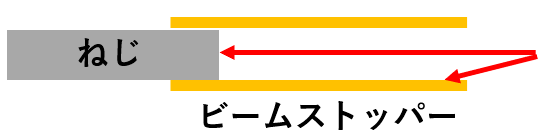
\includegraphics[width=50mm]{picture/setup/stoppermoshi1.png}\\
    \subcaption{ビームを止めるイメージ}
    \label{stmoshi1}
  \end{minipage}
  \begin{minipage}{0.5\hsize}
    \centering
    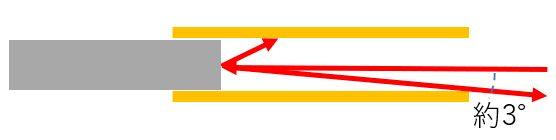
\includegraphics[width=50mm]{picture/setup/stoppermoshi2.png}\\
    \subcaption{ビームストッパー内で反射した場合}
    \label{stmoshi2}
  \end{minipage}
  \caption{ビームストッパーの模式図\cite{2019}}
\end{figure}


\end{document}